\begin{frame}
\frametitle{Evaluation: QEMU Platform \& Limitations}

\textbf{Why QEMU?}
\begin{itemize}
  \item Full system emulation of the RISC-V QEMU VIRT platform
  \item Allows approximating the time each domain runs before scheduling
\end{itemize}

\vspace{0.3cm}
\textbf{Shortcomings:}
\begin{itemize}
  \item No cycle-accurate emulation: microarchitectural state (caches, TLBs, predictors) \textit{not} modeled
  \item Timing channels from shared microarchitectural state cannot be diagnosed
\end{itemize}

\vspace{0.3cm}
\textbf{Implication:} Only constant-time execution paths can be verified. Real hardware with \texttt{fence.t} support (or gem5) is needed to fully evaluate temporal isolation.

\end{frame}

\begin{frame}
\frametitle{Evaluation: Blinky Demo}

Two tasks in separate domains communicating via a Queue:

\vspace{0.2cm}
\begin{center}
\resizebox{0.70\textwidth}{!}{\input{figures/blinky_timeline.tex}}
\end{center}

\vspace{0.2cm}
\begin{itemize}
  \item Sender scheduled at domain tick 4, Receiver at domain tick 2
  \item Round-trip time measured with \texttt{rdcycle}: \textbf{50,000 cycles} $\pm$ \textbf{1 cycle}
  \item Demonstrates constant-time domain switching
\end{itemize}

\end{frame}

\begin{frame}
\frametitle{Evaluation: Multi-Domain Demo}

4 domains, each with a privileged task that creates a higher-priority unprivileged task:

\vspace{0.2cm}
\begin{center}
\resizebox{0.9\textwidth}{!}{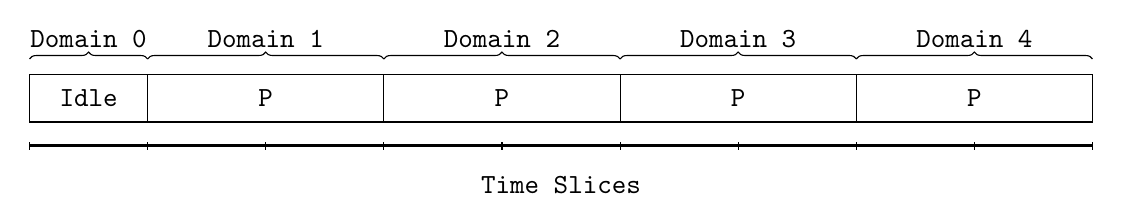
\begin{tikzpicture}[font=\ttfamily]

    % Style for general text nodes
    \tikzset{lbl/.style={inner sep=1pt, align=center}}

    % Define vertical coordinates for rows and labels
    \def\barheight{0.6} % Height of each bar
    \def\vtopprio{1.5}   % Vertical center of the top bar row
    \def\ytimeline{\vtopprio - \barheight} % Vertical position of the minor frames timeline

    % Define standard tick positions
    \def\timeslice{1.5}

    % Domain 0
    \def\tstart{0}
    \def\tend{\timeslice*1}
    \path[draw, decorate, decoration=brace] (\tstart, \vtopprio + 0.5) -- (\tend, \vtopprio + 0.5) node[lbl, midway, above, yshift=0.3em]{Domain 0};
    \draw (\tstart, \vtopprio-\barheight/2) rectangle (\tend, \vtopprio+\barheight/2) 
      node[lbl, midway]{Idle};

    % Domain 1
    \def\tstart{\timeslice*1}
    \def\tend{\timeslice*3}
    \path[draw, decorate, decoration=brace] (\tstart, \vtopprio + 0.5) -- (\tend, \vtopprio + 0.5) node[lbl, midway, above, yshift=0.3em]{Domain 1};
    \draw (\tstart, \vtopprio-\barheight/2) rectangle (\tend, \vtopprio+\barheight/2) 
      node[lbl, midway]{P};

    % Domain 2
    \def\tstart{\timeslice*3}
    \def\tend{\timeslice*5}
    \path[draw, decorate, decoration=brace] (\tstart, \vtopprio + 0.5) -- (\tend, \vtopprio + 0.5) node[lbl, midway, above, yshift=0.3em]{Domain 2};
    \draw (\tstart, \vtopprio-\barheight/2) rectangle (\tend, \vtopprio+\barheight/2) 
      node[lbl, midway]{P};

    % Domain 3
    \def\tstart{\timeslice*5}
    \def\tend{\timeslice*7}
    \path[draw, decorate, decoration=brace] (\tstart, \vtopprio + 0.5) -- (\tend, \vtopprio + 0.5) node[lbl, midway, above, yshift=0.3em]{Domain 3};
    \draw (\tstart, \vtopprio-\barheight/2) rectangle (\tend, \vtopprio+\barheight/2) 
      node[lbl, midway]{P};

    % Domain 4
    \def\tstart{\timeslice*7}
    \def\tend{\timeslice*9}
    \path[draw, decorate, decoration=brace] (\tstart, \vtopprio + 0.5) -- (\tend, \vtopprio + 0.5) node[lbl, midway, above, yshift=0.3em]{Domain 4};
    \draw (\tstart, \vtopprio-\barheight/2) rectangle (\tend, \vtopprio+\barheight/2) 
      node[lbl, midway]{P};

    % Main timeline axis
    \draw[thick] (0, \ytimeline) -- (9*\timeslice, \ytimeline);

    % Intermediate ticks (not all but to give structure)
    \foreach \x in {0, ..., 9} {
         \draw (\x*\timeslice, \ytimeline-0.05) -- (\x*\timeslice, \ytimeline+0.05);
    }

    % Central label below the timeline
    \node[lbl] at ( { 4.5 * \timeslice }, \ytimeline-0.5 ) {Time Slices};

\end{tikzpicture}
}
\end{center}

\vspace{0.2cm}
\begin{itemize}
  \item Domain ticks are deterministic (1, 3, 5, 7, ...)
  \item Priority scheduler still works within each domain
  \item Trade-off: domain-relative delays, added complexity, reduced throughput
\end{itemize}

\end{frame}
